\section{Imported Data Sources}

\begin{longtable}{lllll}
\toprule
 No. & Name  & Measurand & Data Format & URL \tabularnewline
\midrule
\endhead
 1 & Weather Data Stuttgart & Humidity, Temperature, & csv & luftdaten.info \tabularnewline
   & & Pressure & & \\ 
 2 & Luftdaten Brandenburg & O\textsubscript{3}, NO, NO\textsubscript{2}, PM10, & xls & luftdaten.brandenburg.de \tabularnewline
	 & & PM2.5, SO\textsubscript{2}, CO & & \tabularnewline
 3 & Umweltbundesamt & PM10, SO\textsubscript{2}, O\textsubscript{3}, NO\textsubscript{2}, CO & csv &  umweltbundesamt.de \tabularnewline
 4 & Pegel Online & Water Level & REST, & pegelonline.wsv.de \tabularnewline
   & Water Level & & SOAP, HTTP & \tabularnewline
 5 & BLUME & N\textsubscript{2}O, SO\textsubscript{2}, PM10, & HTML & https://www.berlin.de \tabularnewline
	 & & C\textsubscript{6}H\textsubscript{6}, CO, O\textsubscript{3} & & \tabularnewline
 6 & BFS UV-Index & UV-Index & HTML & http://www.bfs.de\tabularnewline
\bottomrule
\end{longtable}

\section{How to Write a Data
Importer}\label{how-to-write-a-data-importer}

\textbf{Authoriship}

\begin{longtable}[]{@{}llll@{}}
\toprule
Version & Date & Modified by & Summary of changes\tabularnewline
\midrule
\endhead
0.1 & 2017-07-29 & Jawid, Rohullah & Initial version\tabularnewline
\bottomrule
\end{longtable}

\vspace*{4mm}

This chapter guides you through building your own importer on top of an
already existing template.

\subsection{Template}\label{template}

Instead of wrting a long manual on how to write an importer we provide
you with starter apps (templates) that you can start to customize right
away.

\subsection{Pre-requisites}

We assume that you are:

\begin{itemize}
\tightlist
\item
  comfortable working with Java and Spring Boot
\item
  already familiar working with Spring Batch
\item
  having knowledge of working with multi module applications using maven
  and Spring Boot.
\end{itemize}

If you need a quick start guide of Spring Batch you can find it
\href{https://projects.spring.io/spring-batch/}{here:}

\subsection{How to Proceed}

\begin{enumerate}
\def\labelenumi{\arabic{enumi}.}
\tightlist
\item
  Download or copy the template that fits your needs.
\end{enumerate}

\textbf{Template Modules}

The template is a multi module application which includes two modules:

\begin{itemize}
\tightlist
\item
  application
\item
  library
\end{itemize}

These modules are defined inside \texttt{pom.xml} file.

\begin{verbatim}
<modules>
        <module>library</module>
        <module>application</module>
</modules>
\end{verbatim}

\begin{enumerate}
\def\labelenumi{\arabic{enumi}.}
\setcounter{enumi}{1}
\tightlist
\item
  Start by changing the importer name inside pom.xml in the root
  directory of the project. You don't need to change anything else
  inside pom.xml.
\end{enumerate}

\begin{verbatim}
<groupId>de.tu_berlin.ise.open_data</groupId>
    <artifactId>your-importer-name-here</artifactId>
    <version>0.1.0</version>
    <packaging>pom</packaging>
\end{verbatim}

\begin{enumerate}
\def\labelenumi{\arabic{enumi}.}
\setcounter{enumi}{2}
\item
  Once you finished editing \texttt{pom.xml} you can open it as a
  project using your IDE. Now you can start to customize it.
\item
  Before changing anything else you can see how the importer works by
  running a kafka server locally and starting the importer's main class
  using your IDE.

  OR

  Inside the root directory of the importer run these commands:

  \$ cd application \$ mvn spring-boot:run
\item
  You can now see inside the console how a simple job runs.
\end{enumerate}

\subsubsection{Things to know about the
template:}\label{things-to-know-about-the-template}

\begin{itemize}
\tightlist
\item
  Inside the \texttt{pom.xml} in the `application' module the following
  dependency is used to include the `library' module:
\end{itemize}

\begin{verbatim}
<dependency>
    <groupId>de.tu_berlin.ise.open_data.library</groupId>
    <artifactId>library</artifactId>
    <version>0.0.1-SNAPSHOT</version>
</dependency>
\end{verbatim}

\begin{itemize}
\tightlist
\item
  Registered beans inside the library module could be autowired by
  importing the `ServiceConfiguration' class from package
  `de.tu\_berlin.ise.open\_data.library'. You can see how it is imported
  in main class:
\end{itemize}

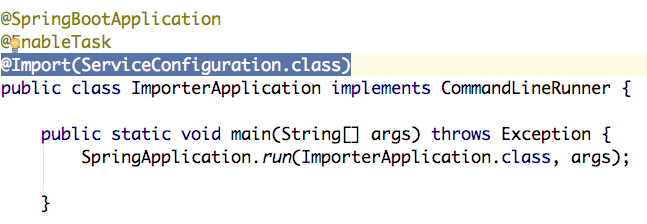
\includegraphics[width=1.00\textwidth]{images/template.png}

You can now start to edit the template.